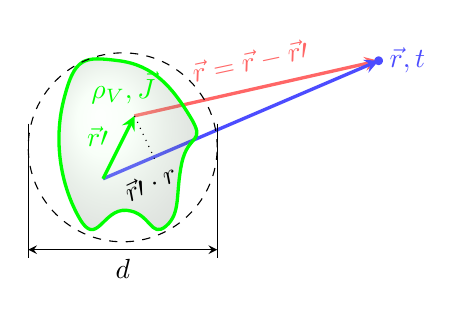
\begin{tikzpicture}[line width = 1.2pt, line join=round,>=stealth]
	% Differenzvektor R
	\draw [->, color=red!60] (1.4,1.8) -- (4.5,2.5);
	\draw [color=red!60] (3.8,2.4) node[anchor=south east, rotate=12] {$\vec{r}  = \vec{r}  - \vec{r}\prime  $};
	% Aufpunkt
	\draw [->,color=blue!70] (1,1) -- (4.5,2.5) node[anchor=west] {$\vec{r} , t$};
	\filldraw [color=blue!70] (4.5,2.5) circle (1pt);
	% Ladungsdichte
	\coordinate (a) at (2.1,1.8);
	\coordinate (b) at (2,1.2);
	\coordinate (c) at (1.8,0.4);
	\coordinate (d) at (1.3,0.6);
	\coordinate (e) at (0.7,0.5);
	\coordinate (f) at (0.5,2);
	\coordinate (g) at (1.2,2.5);
	\shade[ball color=white!10!green!20,opacity=0.20] plot [smooth cycle, tension = 1] coordinates {(a) (b) (c) (d) (e) (f) (g)};
	\draw [color=green] plot [smooth cycle, tension = 1] coordinates {(a) (b) (c) (d) (e) (f) (g)} node [sloped, below] {\ $ \rho_\text{V}, \vec{J} $};
	\draw [->,color=green] (1,1) -- (1.4,1.8);
	\draw [color=green] (1.2,1.8) node[anchor=north east] {$ \vec{r}\prime  $};
	\draw [dotted, thin] (1.4,1.8) -- +(-65:0.6) node[below,rotate=25,xshift=-5]{$\vec{r}\prime \cdot\vu{r}$};
	\draw[dashed,thin] (1.25,1.4) circle (1.2cm);
	\draw[thin] (0.05,1.7) -- (0.05,0);
	\draw[thin] (2.45,1.7) -- (2.45,0);
	\draw[thin, <->] (0.05, 0.1) -- (2.45, 0.1) node[midway, below]{$d$};
\end{tikzpicture}